%@+leo-ver=4-thin
%@+node:rodrigob.20040908003956.1:@thin doc/design.tex
%@@color
%@@language latex

\documentclass{report}
%\documentclass{article}
%\documentclass[A4paper, notitlepage]{article}
                                              
\usepackage[utf8]{inputenc}
\usepackage[english]{babel}
\usepackage{graphicx}
\usepackage{verbatim}

\frenchspacing
\linespread{1} %espacio entre líneas
%\setlength{\parindent}{25pt} %profundidad de la sangría
\setlength{\parskip}{0.7ex plus 0.2ex minus 0.2ex} %espacio entre párrafos

\usepackage{fancyhdr}
\usepackage[sectionbib]{chapterbib}
\usepackage{amsmath}

\usepackage[pdftex]{hyperref}


\lhead{Chalks}
\rhead{\emph{Design proposal}}
\lfoot{}
\cfoot{\thepage}
\rfoot{}

%\usepackage[top=2cm,bottom=2cm,left=2.5cm,right=2.5cm,footskip=1cm,headheight=.5cm,headsep=2cm,textheight=3cm]{geometry}
\usepackage[top=2cm,bottom=2cm,left=2.5cm,right=2.5cm]{geometry}
                                              
\pagestyle{fancy}

\title{\large \emph{Chalks, collaborative text editing for everyone} \\ \huge Design documentation}
\author{Rodrigo Benenson, Ricardo Niederberger}
\date{Technical draft as of\\ \today}

                                           
\begin{document}


\begin{figure}[!t]
 \begin{center}
    
\includegraphics[angle=0,width=5cm]{schemas/logo.jpg}
 \end{center}
\end{figure}


\maketitle
\thispagestyle{empty}

\newpage
\setcounter{page}{1}


\tableofcontents
\newpage
%@+at
% \listoffigures
% %\newpage
% 
% \listoftables
% \newpage
%@-at
%@@c

%@+others
%@+node:rodrigob.20040908172407:Chalks
\chapter{Chalks}


Chalks is a software \emph{under development} for crossplatform realtime concurrent text editing.
The primary focus will be ease of use and minimum requirements.


Chalks is available at \url{http://chalks.berlios.de}


%@+others
%@+node:rodrigob.20040908172407.1:Requirements
\section{Requirements}

These are the requirements for Chalks:

\begin{description}

\item [Realtime Concurrent Edition] \hspace{0cm} \\
    \begin{itemize}
    \item As defined in Chengzheng Sun's works, see the "Research Notes" chapter.
    \end{itemize}
    
\item [Easy to install] \hspace{0cm} \\
    \begin{itemize}
    \item The user should not know about python existence
    \item Lightweight
    \item Ideally only one executable file, without requiring an installation process
    \end{itemize}
    
\item [Easy to use] \hspace{0cm} \\
    \begin{itemize}
    \item Scan local network (also guessing local network) for Chalks servers
    \item Collaborative NotePad for dummies
    \item Very simple gui (figure \ref{fig:chalksguiconcept}), notepad/wordpad look'n'feel, so it should have similar menus and basic features:
      \begin{itemize}
      \item Search, Find, Replace, Print, Save as, Insert date/time.
      \end{itemize}

\begin{figure}[htbp]
 \begin{center}
    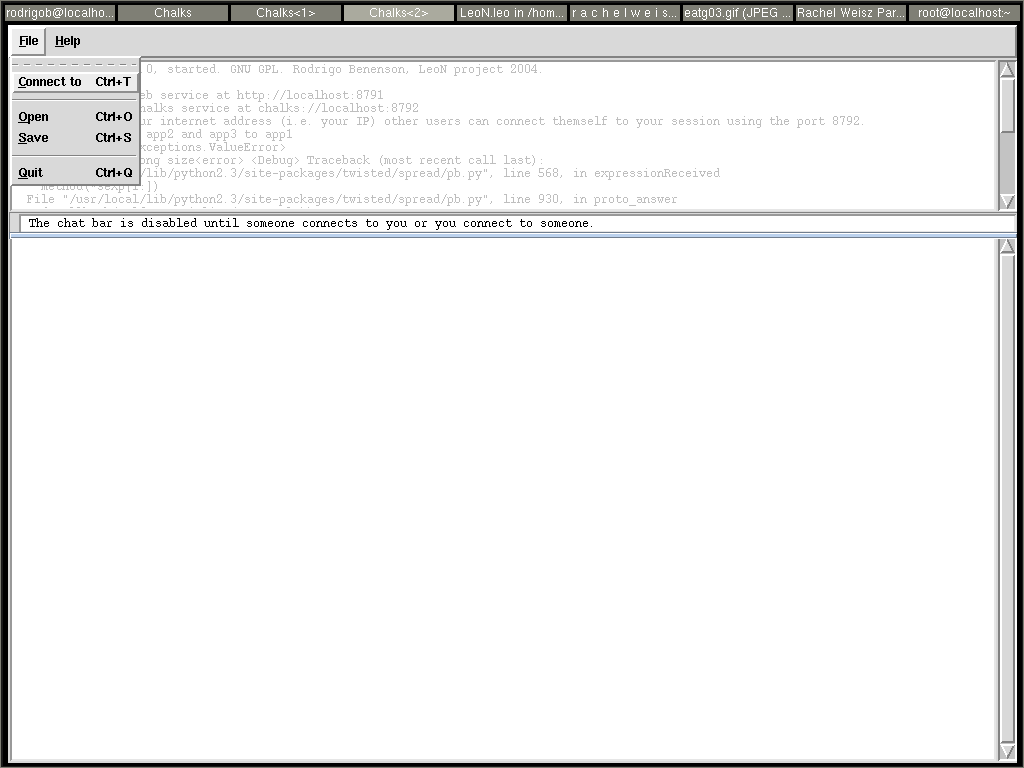
\includegraphics[angle=0,width=0.5\linewidth]{schemas/chalks_gui_concept.png}
 \end{center}
 \caption{Chalks Gui Concept}
  \label{fig:chalksguiconcept}
\end{figure}
      
    \item Undo/redo operations
    \item Chat space among users
    \item Background text coloring for indicating the user who made changes
    \item Cursors for indicating other users current position on the text, as an additional measure to avoid conflicts
    \item Only text, no pretention of text formatting or any multimedia support
    \item One app instance can manage only one document, but can run many instances in a computer. In other words, Single Document Interface approach.
    \item One app instance can do only one thing at a time: connect to a remote server or serve a local file.
    \end{itemize}
    
\item [Descentralized data flow] \hspace{0cm} \\
    \begin{itemize}
    \item Nearby users will have better ping (responsiveness) than remotes one
    \end{itemize}
    
\end{description}
%@nonl
%@-node:rodrigob.20040908172407.1:Requirements
%@+node:rodrigob.20040908172711:Development difficulties
\section{Development difficulties}

The development of Chalks has some specific difficulties, it is important the have them in mind in order to allow reducing risks:

\begin{itemize}
\item Debugging of distributed applications
\item Creating tests for the concurrent editing algorithms
\item Separating GUI frontend from concurrent editing logic in order to ease automatic tests
\end{itemize}
%@nonl
%@-node:rodrigob.20040908172711:Development difficulties
%@+node:rodrigob.20040908172711.1:Aspects
\section{Aspects}

Chalks is a software with three aspects. Identifiying these aspects helps understanding the application structure:

\begin{enumerate}

\item Concurrent Editing (figure \ref{fig:operationsintime})

  \begin{itemize} 
  \item Managing Concurrent Realtime editing of just text 
     \begin{itemize}
     \item Define the memory/cpu performance
           
\begin{figure}[htbp]
 \begin{center}
    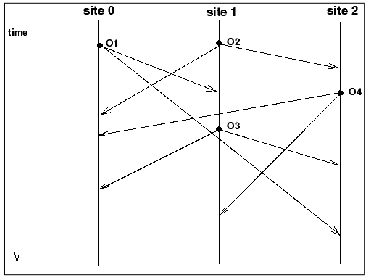
\includegraphics[angle=0,width=0.3\linewidth]{schemas/operations_in_time.png}
 \end{center}
 \caption{Operations in the time}
 \label{fig:operationsintime}
\end{figure}

     \end{itemize}
     
  \item Receive tagged atomic operations over the text and manage them
  \item Generate tagged atomic operations over the local text and pass them to the network layer
  \end{itemize}
  
\item Network

  \begin{itemize}
  \item Create a transparent layer between the concurrent editing of objects
      \begin{itemize}
      \item Creates the ilustion of an "all to all" network (figure \ref{fig:alltoallnetwork})
      
\begin{figure}[htbp]
 \begin{center}
    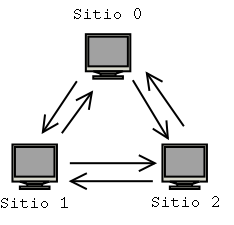
\includegraphics[angle=0,width=0.3\linewidth]{schemas/all_to_all_network.png}
 \end{center}
 \caption{All to all network}
 \label{fig:alltoallnetwork}
\end{figure}
      
      \item Define the real network topology (figure \ref{fig:realnetwork})
\begin{figure}[htbp]
 \begin{center}
    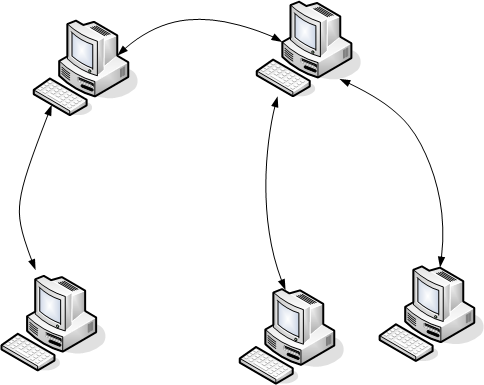
\includegraphics[angle=0,width=0.3\linewidth]{schemas/real_network.png}
 \end{center}
 \caption{A possible real network topology}
 \label{fig:realnetwork}
\end{figure}

      \item Define the protocol
      \item Define the network usage performances
      \end{itemize}
  \item Insertion/deletion of new nodes into the network $\leftarrow$ \emph{tricky point}
  \item How to discover Chalks servers on the current local network automatically    
  
       Figure out local ip address and netmask, then scan ip range for default chalks server port. No need to code everything by hand, we will use the project \href{http://sourceforge.net/projects/pyzeroconf}{Multicast DNS Service Discovery for Python}  by Paul Scott-Murphy.  This module seems impressive, since it's compatible (well, claims to be) with Apple's opensource implementation for Darwin which should be pretty much industry standard. 
       
       There is preliminary support for multicast DNS on Twisted (http://svn.twistedmatrix.com/cvs/trunk/sandbox/itamar/mdns/?root=Twisted), but right now it's very experimental, only suppports querying  and doesn't seem to be evolving fast enough, so \em{pyzeroconf} seems to be the best option.
              
       We also need to think about \href{http://www.iana.org/assignments/port-numbers}{IANA standard port numbers} when coming up with a default server port and registering it on the network with rendezvous.
       
  \item Translation/transport of atomic operations
  \end{itemize}
  
\item Gui

  \begin{itemize}
  \item Simple gui

  \item Reflect the local and remote operations over the seen text (figure\ref{fig:aspectcollaboratingsmallshot})
\begin{figure}[htbp]
 \begin{center}
    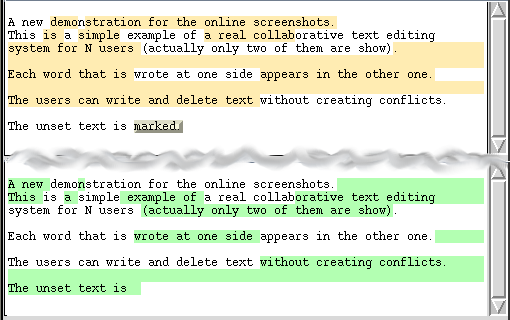
\includegraphics[angle=0,width=0.4\linewidth]{schemas/collaborating_small_shot.png}
 \end{center}
 \caption{Remote users operations are colored}
 \label{fig:aspectcollaboratingsmallshot}
\end{figure}
  
  \item Allow user entry of operations, pass the atomic operations to the Concurrentediting layer $\leftarrow$ \emph{tricky point}
  \end{itemize}
\end{enumerate}
%@nonl
%@-node:rodrigob.20040908172711.1:Aspects
%@+node:rodrigob.20040908172959:Research notes
\section{Research notes}

For definitions of Real-time Cooperative Editing Systems, and their basic properties: Convergence, Casuality-preservation and Intention-preservation and how to achieve them (Search at http://www.researchindex.com for these files and related files):

- \href{http://citeseer.ist.psu.edu/sun98achieving.html}{Achieving convergence, causality-preservation, and intention.. - Sun, Jia et al. - 1998} \emph{$\leftarrow$ the must}

- \href{http://citeseer.ist.psu.edu/sun97generic.html}{A Generic Operation Transformation Scheme for Consistency.. - Sun, Jia (1997)}

- \href{http://citeseer.ist.psu.edu/sun98operational.html}{Operational Transformation in Real-Time Group Editors: Issues, Algorithms, and Achievements (1998)}

- \href{http://citeseer.ist.psu.edu/sun98reversible.html}{Reversible inclusion and exclusion transformation for string.. - Sun, Chen et al. - 1998}

- \href{http://intcomm.wiki.taoriver.net/moin.cgi/RealTimeCooperativeEditingSystemsPaper}{Realtime Collaborative Edition explained in plain English}
%@-node:rodrigob.20040908172959:Research notes
%@-others
%@nonl
%@-node:rodrigob.20040908172407:Chalks
%@+node:rodrigob.20040908172407.2:Design Proposal
\chapter{Design Proposal}

%@+others
%@+node:rodrigob.20040908004801:Introduction
\section{Introduction}

This text covers every defined aspect and proposes a technical solution to implement all requirements.
This is mostly a documentation of the initial Chalks design.


Root concept: \emph{Keep It Simple}, minimal complexity to acomplish the strictly necessary requirements.


%@-node:rodrigob.20040908004801:Introduction
%@+node:rodrigob.20040908010357:Concurrent Editing
\section{Concurrent Editing}

Direct implementation of the linear undo/redo algorithm described in Chengzheng Sun's works. This algorithm is the simpler aviable. It has a good compromise in the memory/cpu usage, with a some charge on the memory. Anyway as the objects managed are strings, the memory rarely grows more than a few tens of megabytes.

Chengzheng Sun's algorithm defines three objects: the operations, the history buffer (HB), and the resulting text.

\em{Operations} are specific transformations over the text (insertion, deletion) originated from a specific version of the text. The \em{history buffer} is a buffer of all the operations applied over the text. And the resulting text is the product of applying all the HB operations over the original text.

The concurrent editable algorithm defines what to do with a new operation. The processing of the received operation will have effect over the HB and over the original resulting text.


\begin{figure}[htbp]
 \begin{center}
    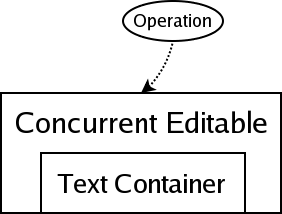
\includegraphics[angle=0,width=0.5\linewidth]{schemas/concurrent_editable.png}
 \end{center}
 \caption{ConcurrentEditable, TextContainer and the Operations}
 \label{fig:concurrenteditable}
\end{figure}

\fbox{\begin{minipage}[c]{\linewidth}
\emph{Note}: the actual WIP version does not separate in a clear enough way the TextContainer from the ConcurrentEditable object. I think this separation should be enforced to ease later integration with GUI
\end{minipage}}

Using Python power the operations can be easilly represented as objects, following an easy API similar to Chengzheng Sun's notation.

In a similar way the Concurrent Editable algorithm can be implemented as an almost direct translation from the Chengzheng Sun papers to python code.

The {\texttt TextContainer } class is a simple one that contain an unicode string, and have methods for insertion, deletion of chars and the retrieval of the actual content.
%@-node:rodrigob.20040908010357:Concurrent Editing
%@+node:rodrigob.20040908010357.1:Network
\section{Network}

The definition and implementation of the networking system is the most difficult aspect of the software. Distributed bugs arises and issues not covered in the papers have to be afronted.

Essentially the network has to take care of three things:
\begin{itemize}
\item Sent operations have to arrive to every connected user
\item If a new user logs in, everyone has to know about it
\item If a user logs out, everyone has to know about it
\end{itemize}

Every operation has a specific identifier. This identifier is the number of operations that the emitter site has received from other sites (including himself). This identifier defines without ambiguity the *version* of the document over which the operation was generated.

To simplify the implementation instead of enumerating the sites (as in the paper) the sites are individualized by an unique id (ip+port). Then the operations are tagged with a dictionary of the kind {\texttt {id1: ops\_from\_id1, id2: ops\_from\_id2, ...}} (including site own id).

This approach becomes less efficient if many sites just connect once, send an operation and then disconnect, but this is a rare case. This approach is less efficient than using an ordered list, but it is simpler and functional. It is simpler because we do not care about the order of arrival, the disconnections and reconnections, and when new users are added to the session the management becomes trivial.

%@+others
%@+node:rodrigob.20040908012337:Topology
\subsection{Network topology}

Following the KIS principle which is the simplest network architectures that does the job fine ?

The proposal is to use a ``Connect to One, Accept N'' topology, also known as a ``simple tree''. See the image \ref{fig:connectooneacceptN} to get an idea.    

\begin{figure}[htbp]
 \begin{center}
    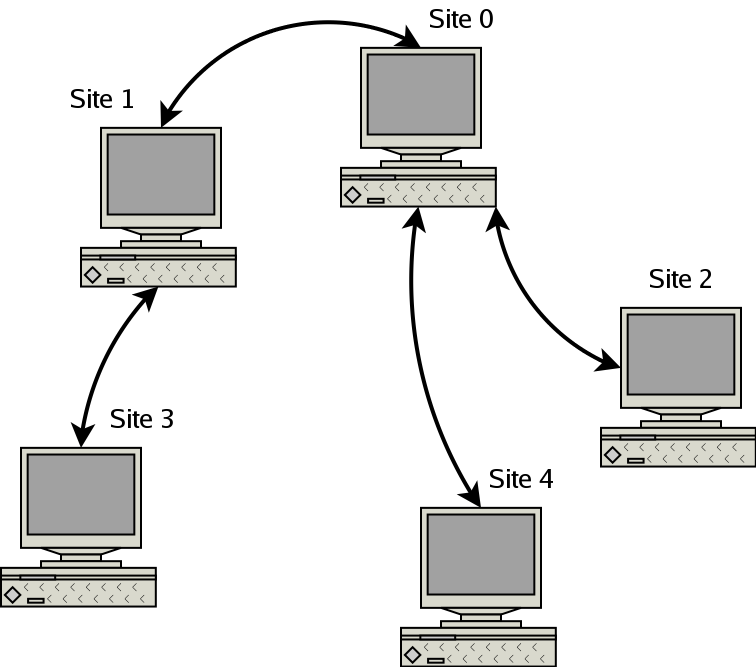
\includegraphics[angle=0,width=0.5\linewidth]{schemas/connect_to_one_accept_N.png}
 \end{center}
 \caption{Connect to One, Accept N ilustrative topology}
 \label{fig:connectooneacceptN}
\end{figure}

The concept of this topology is, very simple. One user only want to connect himself to one computer, so let's do that. If more than one user want to connect to the same computer let's do that. After the first connection no more connections are made.

This is topology is inefficient. In the figure, when site 4 edit the text, the operation will be relayed by site 0 and site 1, adding inecessary delays. This is true, but this topology is very simple implement. It has also an interesant advantage, it gives to the users the control of the network. In the figure, if sites [0,2,4] are in the same LAN, and sites [1,3], in another one, then the topology is not so bad. Also if an user is working in a slow connection (example, low SNR wireless conneciton), it would prefer to have only one connection to the nearest (in ping measure) machine. Having more than one connection add transfers costs to keep the TCP/IP links alive. If the users control the conection they can choose the computer with overload. A tipical user case will be simply N-to-One (central server receiving all the conections).
 
The tree topology is not only simple to implement but also simple to analyse.
    
When a site receives an operation it applies it locally and spread it to all the other known sites, excluding the node that sent the operation. As the topology is an acyclic graph, no special precautions has to be taken (to avoid repeated reception).

Let's see what should happen when a user connects himself to a session.
\begin{itemize}
\item New user enters the network

A user has choosen a machine to connect to. This machine receives a new connection and has to send back, the current text and the HB. We have to take care of new operations that could be generated during the connection process.

Chengzheng Sun's algorithm includes a purge procedure to avoid the HB getting unncessarily big.

This HB purge could be implemented as a method which calls itself repeatedly, using a call like "reactor.callLater(self.HBPurge(), purgeDelay)". This "service method" pattern could repeat a lot on such networked application, especially when using a networking framework like Twisted, with deferred execution.

Upon the first text editing, the new user will generate an operation with a new entry in the tag. When a site receives it for the first time it will include it in the list of know sites. If a received operation does not include (not a key in it's id->version map) a known site id, obviously this node has received zero operations from that site.


\item A user quits the network

No special precaution has to be taken when a user quits. We have to simply disconnect from the parent node, and kill all children nodes. This will create a cascade that will close the branch adequately.


\fbox{\begin{minipage}[c]{\linewidth}
\emph{Note}: this could be an inconvenience, depending of the usage scheme. Maybe we could create a transaction system to invite all children nodes to connect themself to the parent node. But synchronisation issues may arise (``what if a packet arives to the parent while children-childrens are connecting to them ?''). This is a non trivial topic that we should check. For an initial implementation branch die seems fine to me, but is it the desired behaviour ? (let's check the requiriment)
\end{minipage}}

      
HB purge should also purge sites info. If a site id does not appear more in the HB, then it should be deleted from the known sites list, thus shrinking back the packet sizes since no memory traces are keep in any connected site.
\end{itemize}
%@nonl
%@-node:rodrigob.20040908012337:Topology
%@-others

\subsection{Protocol}

{\texttt Operation} objects serialized and transfered via Twisted Spread.

\begin{itemize}
\item Well documented API
\item Simple and eficient binary serialization (low bandwith usage)
\item Well documented Serialization protocol (Banana)
\item Fast serialization (C modules)
\item Pythonic
\end{itemize}

\subsection{API}
  
\href{http://www.twistedmatrix.com}{Twisted}

\begin{itemize}
\item Well documented API
\item Full featured, spread, authentication, web services, diverse protocols, etc.
\item Pythonic
\item Easy to embed in the software distribution
\end{itemize}
%@nonl
%@-node:rodrigob.20040908010357.1:Network
%@+node:rodrigob.20040908010357.2:Gui
\section{Gui}

Show the text container, generate new operations over the text, allow sending chat messages to the other users.

The idea is to provide to the user all what it need to see in only one window, splitted in two areas: the text area and the chat area.

\begin{figure}[htbp]
 \begin{center}
    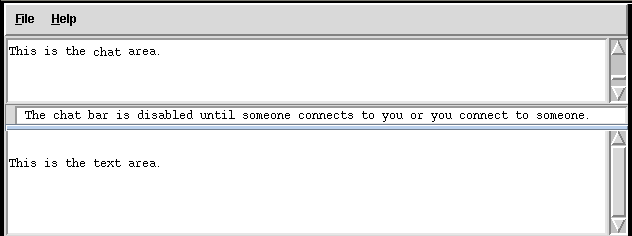
\includegraphics[angle=0,width=0.5\linewidth]{schemas/text_and_chat_area.png}
 \end{center}
 \label{fig:textandchatarea}
 \caption{Text and chat areas in the same window}
\end{figure}

  
The chat area is used as a log window, to receive message, and have an input section to send messages. This input section can also be used to enter advanced commands (to enable/disable debug logs, to select special options, etc...). Different colors in the chat bar are used to differenciate diferent kind of messages.

The chat area is resizable (click and drag). If  it is totally colapsed it transform itself into a status bar, that show the last line in the chat area.

\begin{figure}[htbp]
 \begin{center}
    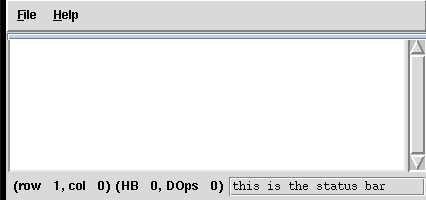
\includegraphics[angle=0,width=0.5\linewidth]{schemas/colapsable_chat_area.png}
 \end{center}
 \label{fig:colapsablechatarea}
 \caption{The chat area is colapsable, transforming itself in a normal status bar}
\end{figure}


In the text area color codes are used to differenciate the users entries. Also the local entry are marked in such a way that the local user know when a group of chars have been sent or not.


\begin{figure}[htbp]
 \begin{center}
    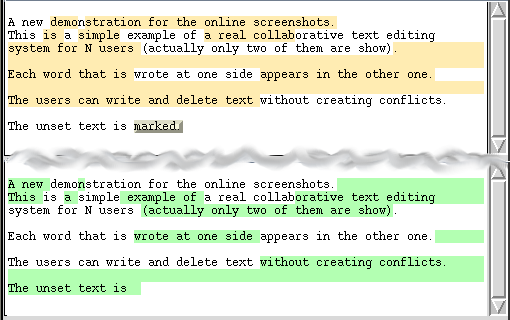
\includegraphics[angle=0,width=0.5\linewidth]{schemas/collaborating_small_shot.png}
 \end{center}
 \caption{Text from other users are colored. Text not yet processed is raised}
 \label{fig:collaboratingsmallshot}
\end{figure}


The color of the users is randomly choosen at the local site. The color generator choose in a family of smooth agradable colors. 


\subsection{Menus}

The menus should be strictly minimal, siilar to NotePad ones, but with less options.
The number of dialogs is also minimal, and they complexity very low.

\begin{figure}[htbp]
 \begin{center}
    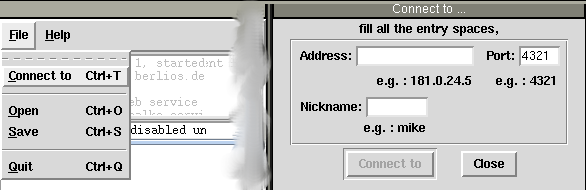
\includegraphics[angle=0,width=0.5\linewidth]{schemas/simples_menus_and_dialogs.png}
 \end{center}
 \caption{Simples menus and dialogs}
 \label{fig:simplesmenusanddialogs}
\end{figure}


\subsection{API}

\href{http://www.python.org/topics/tkinter/}{Tkinter}

\begin{description}
\item [Pros]
    \begin{itemize}
    \item Easy to include in the python distribution
    \item Ligthweigth (? compared to wxwindows ?)
    \item Python default gui, crossplatform
    \item Good coloring facilities
    \item Documented, easy API
    \item Full Unicode support
    \item Stable API
    \end{itemize}

\item [Cons]
    \begin{itemize}
    \item Manage text as a bidimensional object
    \item Ugly: The gui is not similar to the OS default one (this may \href{http://tcl.projectforum.com/tk/47}{change} in the future)
    \item Low mindshare among other programmers, wxPython seems to be the mainstream python gui programming toolkit nowadays
    \item Increasingly few projects using it and as such there is less people reporting bugs, etc. (development is not too active lately)
    \item But anyway we believe we should keep on using tkinter for the first release and see how things play along. Provided we honour our intent of keeping GUI code clearly separated from concurrent/networking code, we should be safe
    \end{itemize}
\end{description}

\fbox{\begin{minipage}[c]{\linewidth}   
\emph{Note}:the gui code implementation should be as well defined and separated as possible to allow future implementations using diferent gui engines (natives, scintilla, etc.)
\end{minipage}}
%@nonl
%@-node:rodrigob.20040908010357.2:Gui
%@-others
%@nonl
%@-node:rodrigob.20040908172407.2:Design Proposal
%@+node:rodrigob.20040913234027:Notes
\chapter{Notes}

Misceleanous notes about sections or aspects of the code.

%@<<about the connections process>>
%@+node:rodrigob.20040913233519:<<about the connections process>>
%@@language latex
%@@color
\section{About the connections process}

The Children start a connection. The ChalksNode object request a connection to the parent. 

The parent receive access to the children as a reference to ChalksNode and the children gets access to the parent obtaining access to a ChalksAvatar instance created in the parent side.

ChalksNode can receive calls to the remote\_ (view\_ ) methods.
ChalksAvatar can receive calls to the perspective\_ methods.

We want the childrens able to call the ChalksNode methods. Thus when the Childrens call the collaborate\_in using his avatar on the parent side, he receive back (in a huge list of params) the parents ChalksNode reference.

The connection process occurs in this order:
\begin{enumerate}
\item ChalksNode require a connection to the parent using the {\texttt connect\_to\_parent} method. Thus a parent ChalksAvatar object is created and passed to the parent as an access to the Children. This parent ChalksAvatar instance has no {\texttt mind} object.

\item The parent receive through his {\texttt ChalksRealm} the children connection request. A children ChalksAvatar instance is created in the parent side. The parent return to the children a reference to this avatar.

\item The children receive this reference (at {\texttt logged\_in}) and register it as the parent perspective (the access of the children to the parent side). It also register this perspective as the mind of the children side parent ChalksAvatar instance.

\item Now that the children is connect he call in the parent (througth his avatar in the parent side, i.e. throught the parent perpespective) the {\texttt collaborate\_in} method.

\item The parent receive the call, register the children perspective (local children avatar mind) as one more site in the collaboration session and return to the children all the required information to start collaborating.

\end{enumerate}

It worth noting that the ChalksNode object keep only \emph{remote references} of the avatars (of the parent and of the children). When a node call a remote method in the called node receive a call from the local Avatar instance. Thus \emph{the mind} of the local Avatar is compared to the childrens and parents remote references. For a clear example look at the {\texttt send\_message} ChalksNode method.
%@-node:rodrigob.20040913233519:<<about the connections process>>
%@nl
%@+others
%@-others
%@nonl
%@-node:rodrigob.20040913234027:Notes
%@-others

\end{document}
%@nonl
%@-node:rodrigob.20040908003956.1:@thin doc/design.tex
%@-leo
